\documentclass[handout,final,xcolor=dvipsnames]{beamer}

\useinnertheme{rectangles}
\usecolortheme[RGB={140,206,150}]{structure}
\useoutertheme{infolines}
%\setfootline{\insertinstitute,\insertauthor, \hfill slide \insertframenumber/\insertotalframenumber}
\usetheme[height=12mm]{Darmstadt}

\definecolor{lightblue}{RGB}{217,244,212}

\setbeamertemplate{blocks}[rounded]

%\setbeamercolor{block title}{fg=White,bg=Red}
\setbeamercolor{block body}{bg=lightblue}

%\useoutertheme[footline=authortitle,subsection=false]{miniframes}
%\usepackage{pgf,pgfpages}
%\pgfpagesuselayout{resize to}[a4paper,landscape,border shrink=5mm]
\usepackage{xcolor}
\usepackage{booktabs}
\usepackage{fontenc}
\usepackage[utf8]{inputenc}
\usepackage{hyperref}
\hypersetup{colorlinks=false,
linkcolor=blue,
citecolor=red,
urlcolor=blue}


\author{Sebastián Freille (UNC-UCC)}
\title{Universidad Nacional de La Plata (UNLP) \\
  Maestría en Finanzas Públicas Provinciales y Municipales \\ La
  Política de las Finanzas Públicas \\ Clase 9-10}
\date{}
\institute{}


\AtBeginSection[]{
    \begin{frame}
    \vfill
    \centering
    \begin{beamercolorbox}[sep=8pt,center,shadow=true,rounded=true]{title}
        \usebeamerfont{title}\insertsectionhead\par%
    \end{beamercolorbox}
    \vfill
    \end{frame}
}


\begin{document}
\maketitle


\section{Instituciones}

\begin{frame}\frametitle{Un cuento de dos ciudades}
 \begin{figure}[htbp]
    \centering
\includegraphics[scale=0.15]{nogales2008}
   \caption{Un cuento de dos ciudades: el caso de Nogales}
  \end{figure}
\end{frame}


\begin{frame}\frametitle{Un cuento de dos ciudades (cont.)}
\begin{block}{El caso de las dos Nogales}
La ciudad de Nogales es una ciudad de frontera. Una mitad pertenece a
Arizona (USA), la otra mitad a Sonora (MEX). Nogales (USA) tiene un
PBI per capita de 30k, la mayoría de los adultos tienen título
secundario, la mayoría de los adolescentes asisten a la
escuela, las tasas de crimen son bajas y la corrupción e ineficiencia
son relativamente bajas. Nogales (MEX) tiene un PBI per capita de 10k,
la mayoría de los adultos no tiene titulo secundario y muchos adolescentes no
asisten a la escuela,  las tasas de crimen son muy altas y la corrupción y la
ineficiencia son relativamente altas. 
\end{block}
\end{frame}


\begin{frame}\frametitle{Reglas del juego y juego del juego}
\begin{itemize}\itemsep 15pt
\item Instituciones (económicas, políticas, sociales) representan las \textit{reglas del juego} que
  agentes juegan. No hay una definición aceptada y general en las
  ciencias sociales. 
\item En palabras de Douglas North, ``las instituciones son las reglas
  del juego y los métodos de hacerlas valer y los actores
  (organizacions) son los equipos que juegan el juego''.
  \item En este enfoque, las instituciones como reglas del juego
    podían ser formales, informales y normas de comportamiento
\end{itemize}
  \end{frame}


\begin{frame}\frametitle{Tipos de instituciones}
\begin{itemize}\itemsep 15pt
\item Una clasificación
\begin{itemize}\itemsep 15pt \medskip
\item Instituciones económicas extractivas $\longrightarrow$ determinan las ``reglas
  económicas del juego'' --ausencia de ley y orden; derechos de
  propiedad inseguros; barreras a la entrada; regulaciones que
  previenen funcionamiento de mercados
  \item Instituciones políticas extractivas $\longrightarrow$
    absolutismo (límite). En general, aquellas que concentran el poder
    en pocas manos, sin efectivos controles y ``checks and
    balances''.
    \item Instituciones económicas inclusivas $\longrightarrow$ ley y
      orden; derechos de propiedad definidos; soporte de mercados y
      Estado al mercado; libre entrada a mercados; acceso a educación
      e igualdad de oportunidades
      \item Instituciones políticas inclusivas $\longrightarrow$
        pluralismo (participación amplia); existencia de ``checks and
        balances''; algun grado de centralización política.
\end{itemize}
\end{itemize}
\end{frame}




\begin{frame}\frametitle{Tipos de instituciones (cont.)}
\begin{itemize}\itemsep 15pt \medskip
\item Otra clasificación
\begin{itemize}\itemsep 15pt \medskip
\item Instituciones predatorias (malas) $\longrightarrow$ aquellas que
  no alientan la inversión y el desarrolo económico. 
\item Instituciones promotoras del desarrollo (buenas)
  $\longrightarrow$ aquellas que permiten y estimulan la inversión y
  el crecimiento. 
\end{itemize}
\end{itemize}
\end{frame}



\begin{frame}\frametitle{Instituciones y poder político}
\begin{itemize}\itemsep 15pt
\item Diferentes conjuntos de instituciones crean diferentes grupos de
  ganadores y perdedores. 
\item ¿Cómo decide una sociedad el conjunto de instituciones de
  equilibrio? ¿Es una alternativa viable la compensación (de ganadores
  hacia perdedores?
\item La clave es el concepto de ``poder político'', entendido en
  contexto democrático. Dos tipos de poder político: 1) de iure; 2) de
  facto. 
\item Instituciones de equilibrio resultado de la suma de ambos tipos
  de poder político. 
\end{itemize}
\end{frame}

\begin{frame}\frametitle{Instituciones ineficientes pero estables?}
\begin{itemize}\itemsep 15pt
\item Suponemos una situacion donde alguien detenta el poder político
  total:
\begin{itemize}\itemsep 15pt \medskip 
\item Problema de \textit{hold-up}: Político en el poder no puede comprometerse a no bloquearlo una
  vez que la inversión este hecha $\longrightarrow$ los productores no
  invertiran
\item Perdedores políticos: el riesgo de perder poder político
  disminuirá el incentivo a adoptar instituciones eficientes
\item Perdedores económicos: diferentes instituciones implican
  diferentes distribuciones de riqueza/ingresos. Ir de ``malas'' a
  ``buenas'' instituciones implica perdedores económicos
  $\longrightarrow$ motivos para bloquear.  
\end{itemize}
\end{itemize}
\end{frame}


\begin{frame}\frametitle{Implicancias}
\begin{itemize}\itemsep 15pt
\item Situaciones donde hay restricciones al poder político (balance
  de poder, división de poderes) mas factibles de producir
  instituciones protectoras de derechos de propiedad amplios. 
\item Si el poder está distribuido entre varios grupos con
  posibilidades de inversión, mas factible que surjan ``buenas''
  instituciones
\item Cambios institucionales que no amenacen el poder político actual
  tienen mas chances de ocurrir. 
\end{itemize}
\end{frame}


\begin{frame}\frametitle{Dinámica del sistema}
  \begin{figure}[htbp]
    \centering \vspace{-3cm}
    \includegraphics[scale=0.5]{ar1}
    \caption{Dinamica del sistema}
    \label{fig:ar1}
  \end{figure}
\end{frame}


\begin{frame}\frametitle{Dinámica del sistema (cont.)}
\begin{itemize}\itemsep 15pt
\item Variables de ``estado'' $\longrightarrow$ instituciones
  políticas y distribución de recursos. Dos motivos:
\begin{itemize}\itemsep 15pt \medskip 
\item Cambian relativamente poco en el tiempo
\item Determinan instituciones económicas y resultados directa e
  indirectamente. 
\end{itemize} 
\item Efecto directo $\longrightarrow$ si las instituciones políticas
  dan todo el poder a un individuo/grupo dificil tener instituciones
  económicas ``buenas''
\item Efecto indirecto $\longrightarrow$ las instituciones políticas
  determinan la distribución de poder de iure; y esto determina
  instituciones economicas y resultados
\end{itemize}
\end{frame}



\begin{frame}\frametitle{Dinámica del sistema (cont.)}
\begin{itemize}\itemsep 15pt
\item Pero no sólo las instituciones económicas son endógenas. Las
  instituciones políticas también lo son $\longrightarrow$
  transiciones democráticas; reformas constitucionales;
\item Distribución del poder político principal determinante de
  instituciones políticas. Formal:
\begin{itemize}\itemsep 15pt \medskip 
\item $IP_{t}$ $\longrightarrow$ $PPdI_{t}$ $\longrightarrow$
  $IP_{t+1}$. Pero $PPdF_{t}$ $\longrightarrow$ $IP_{t+1}$
\end{itemize} 
\item Suele suceder en revoluciones, crisis, y ante amenazas de
  revuelta. 
\end{itemize}
\end{frame}




\begin{frame}\frametitle{¿Las instituciones realmente importan?}
\begin{itemize}\itemsep 15pt
\item Hace algunas décadas, existía prácticamente un consenso
  generalizado $\longrightarrow$ las instituciones importan
  \item Al mismo tiempo, desde esa época, muchisimos trabajos
    adjudicaban a las instituciones políticas (económicas) un rol
    fundamental en la explicación de los diferentes resultados entre
    los países --i.e. volviendo a la primer parte de la materia, los
    intereses/preferencias pasan a segundo plano
    \item Esta visión fue incluso adoptada por organismos
      internacionales y multilaterales $\longrightarrow$ consenso de
      Washington; reformas estructurales e institucionales en países
      subdesarrollados
      \item Sin embargo, dos problemas persistían: 1) no podría
        explicar resultados diferentes de implementar mismas
        instituciones en paises diferentes; 2) no podría explicar si
        son verdaderamente las instituciones las que determinan resultados
\end{itemize}
\end{frame}


\begin{frame}\frametitle{Instituciones endógenas}
  \begin{block}{Instituciones y condiciones}
    Un juego de basket. Dos equipos. Un conjunto universal de reglas y
    un referee imparcial. Un equipo todos miden 210cm, el otro
    180cm. El resultado de este juego esta predeterminado. Las reglas
    del juego (instituciones) tratan a todos por igual pero la
    diferencia (resultado) se da en los recursos que cada equipo trae
    al juego $\longrightarrow$ poder bruto, pre-institucional. SALIDA:
    ¿Y si cambiamos reglas (ajustamos altura de los aros para igualar
    condiciones? ¿Existirán condiciones para que ambos equipos acepten
    esto? Y si esto se así, las instituciones (nuevas) serán estables (self-enforcing)?
    \end{block}
    \begin{block}{Argentina}
El problema con Argentina es que no tiene una justicia
independiente. Pues bien, pongamos una justicia independiente y
aseguremos los derechos de propiedad y el maná caerá del cielo
$\longrightarrow$ Wrong
\end{block}
\end{frame}

\begin{frame}\frametitle{Instituciones endógenas (cont.)}
\begin{itemize}\itemsep 15pt
\item Problema principal $\longrightarrow$ si \textbf{diferentes
    instituciones} son posibles sólo bajo \textbf{diferentes
    condiciones/situaciones}, ¿cómo podemos saber si lo que importa
  realmente (en el sentido causal) son las instituciones o las
  condiciones/situaciones?
  \item Ejemplo $\longrightarrow$ observancia y acatación de
    resultados electorales por parte de partidos políticos.
    \item Cuando un partido A gana una elección, por qué los
      identificados con el partido B aceptan el resultado? ¿No tendrían
      incentivo a no acatar el resultado y tratar de usar la fuerza?
\end{itemize}
\end{frame}


\begin{frame}\frametitle{Instituciones endógenas (cont.)}
\begin{block}{Condorcet sobre el origen de la autoridad}
Cuando la práctica de acometer a todos los individuos a la
  voluntad de la mayoría se introdujo en las sociedades, y cuando los
  ciudadanos empezaron a mirar la decisión de la mayoría como la
  voluntad de todos, no fue porque adoptaron ese método para evitar
  errores y conducirse en base a decisiones basadas en la verdad, sino
  que descubrieron que en miras a la paz y bienestar generales, era
  necesario otorgar autoridad donde la fuerza estaba.
\end{block}
\begin{itemize}
\item La pregunta subsiste: ¿por qué los ganadores y perdedores
  observan las reglas? ¿Estan obedeciendo reglas o están haciendo lo
  que hubieran hecho incluso si no hubieran existido esas reglas?
  \end{itemize}
\end{frame}



\begin{frame}\frametitle{Instituciones endógenas (cont.)}
\begin{itemize}\itemsep 15pt
\item Evidencia $\longrightarrow$ en los países ricos, tanto los
  ganadores como los perdedores respetan los resultados de las
  elecciones; en los países pobres en general, pueden respetarlos o
  no.
  \end{itemize}
  \begin{block}{Elecciones arregladas}
    Una elección muy pareja en Costa Rica en 1948 (PBI per capita 1500
    dolares). Sospechas de fraude. El congreso dio por ganador al
    partido con menos votos. Hubo revueltas y 3000 muertos. Otra
    elección muy pareja en otro país (PBI per capita 20000
    dolares). La Corte Suprema (elegida en parte por el padre de uno
    de los candidatos) dio por ganador al partido con menos
    votos. Cada uno se fue a su casa a en sus minivans a sentarse en
    el jardin. Los tenían por el alto ingreso per capita. 
  \end{block}
 \end{frame}


\begin{frame}\frametitle{El problema del ``commitment''}
\begin{itemize}\itemsep 15pt
\item ¿No sería más eficiente resolver el conflicto de intereses a
  través de una negociación/acuerdo entre las partes? Sería posible si
  no existiera el problema del ``commitment''. 
\item Los grupos en el poder no pueden comprometerse a no usar su
  poder para cambiar instituciones en su favor --ie. promesas campaña Menem
\item Problema de inconsistencia inter-temporal $\longrightarrow$
  aquellos que toman las decisiones hoy no pueden comprometerse a
  ciertas instituciones economicas en el futuro dado que serán
  (posiblemente) otros los que tengan el poder. Por eso cambian
  instituciones hoy --i.e. CFK reforma judicial. 
\end{itemize}
\end{frame}





\begin{frame}\frametitle{Instituciones: resumiendo}
\begin{itemize}\itemsep 15pt
\item Las instituciones importan $\longrightarrow$ influyen sobre las
  normas, las creencias y los resultados. 
\item Las instituciones son endógenas $\longrightarrow$ el tipo y
  funcionamiento de las 
  instituciones dependerá de la configuracíon de intereses y de las
  condiciones de las que surgen
\item Condiciones $\longrightarrow$ Instituciones $\longrightarrow$
  Resultados. Formalmente: $R=f(I)=f(f(C))$
\item Entonces, ¿importan las instituciones?. Si es asi, ¿cuánto?
\end{itemize} 
\end{frame}



\section{Aplicaciones - Casos de ilustración}

\begin{frame}\frametitle{Caso I: Del medioevo a la revolución industrial}
\begin{itemize}\itemsep 15pt
\item El $PPdI$ y $PPdF$ estaba en manos de los Reyes y los derechos
  de propiedad respondían a sus intereses. Instituciones económicas
  atentaban contra la inversión y la tecnología. Perjudicó el
  crecimiento pero aumentó el poder económico de reyes. 
\item En siglo XVII grandes cambios en $IP$ y $IE$ $\longrightarrow$
  cambios en tenencia de tierras y comercio atlántico aumentó $PPdF$
  y poder militar de otros grupos --guerra civil inglesa y revolución
  gloriosa. 
\item Cambios en $IP$ que redujeron el $PPdF$ del rey e introdujeron
  derechos de propiedad de terratenientes y dueños de capital. Proceso
  de crecimiento sostenido culminado en la RI. 
\end{itemize}
\end{frame}


\begin{frame}\frametitle{Caso II: El respeto a las elecciones}
\begin{itemize}\itemsep 15pt
\item La institución de elegir via elecciones
\item Si todos los hombres fueran iguales e igualmente fuertes, ¿por qué los perdedores aceptan el resultado? Porque lo dice la
  Constitución? Porque serían derrotados (por la fuerza) si no lo
  hicieran?
\item Refinando la pregunta $\longrightarrow$ los perdedores actuarían
  de la misma manera (acatando el resultado) si no existiera la
  institución legal?
\begin{itemize}\itemsep 15pt \medskip
\item No siempre. Evidencia sugiere que el ajustarse a las
  instituciones depende de la riqueza del país --cfr casos de fraudes
  en dos países [Przeworski (2004)]
\item Misma institución, diferentes condiciones $\longrightarrow$
  diferentes resultados. 
\end{itemize}
\end{itemize}
\end{frame}



\begin{frame}\frametitle{Caso III: Historia colonial como determinante
  de desarrollo}
\begin{itemize}\itemsep 15pt
\item ¿Por qué no todos los países se desarrollaron? Algunas
  explicaciones posibles: geografía; instituciones; cultura; otras
  (``policies'')
  \item ¿Por qué pueden variar las instituciones? Geografía,
    accidentes históricos, ideas...y por qué persisten esas
    diferencias
  \item Hay basicamente dos tipos de explicaciones. La primera,
    asigna a la geografía y a los accidentes históricos impacto sobre
    elección y persistencia institucional. La segunda, a la cultura.
    \item Acemoglu, Robinston \& Johnson (2001) y Nunn (2008) son
      ejemplos de la primera. Clark (1987), ejemplo de la segunda.
    \end{itemize}
\end{frame}



\begin{frame}\frametitle{Caso III: Historia colonial como determinante
  de desarrollo (cont.)}
\begin{itemize}\itemsep 15pt
\item Acemoglu, Robinson \& Johnson $\longrightarrow$ la mortalidad potencial de
  los colonos (colonizadores/inmigrantes) influyó sobre la estrategia
  colonizadora lo que influyó sobre las instituciones
  \item En lugares donde la mortalidad potencial de colonos era
    baja, se desarrollaron colonias de inmigrantes (instituciones
    inclusivas). Pero donde la mortalidad era alta, se instalaron
    colonias extractivas (instituciones extractivas).
    \item En otras palabras, la mortalidad --condiciones
      preexistentes-- influyó sobre el tipo institucional adoptado. 
    \end{itemize}
\end{frame}


 \begin{figure}[htbp]
    \centering \vspace{1cm}
    \includegraphics[scale=0.3]{arj1}
    \caption{Mortalidad de colonos y riesgo de expropiación}
    \label{fig:arj1}
  \end{figure}
\end{frame}


\begin{frame}\frametitle{Caso IIIA: Los efectos de la esclavitud}
\begin{itemize}\itemsep 15pt
\item Nunn usa datos sobre embarques con numero estimado de esclavos
  de cada ciudad costera de Africa
  \item Supone que los esclavos embarcados en un determinado país son
    de ese país o de países directamente colindantes
    \item Posibles errores de medición (esclavos del interior más
      mortalidad, etc)
      \item También tienen posibles casos de sesgos $\longrightarrow$
        areas menos desarrolladas mas afectadas por comercio de
        esclavos. Controlar por esto. x
    \end{itemize}
\end{frame}



\begin{frame}\frametitle{Caso IIIA: Los efectos de la esclavitud (cont.)}
   \begin{figure}[htbp]
    \centering \vspace{0cm}
    \includegraphics[scale=0.3]{nunn1}
    \caption{Embarques de esclavos}
    \label{fig:ar1}
  \end{figure}
\end{frame}


\begin{frame}\frametitle{Caso IIIA: Los efectos de la esclavitud (cont.)}
   \begin{figure}[htbp]
    \centering \vspace{0cm}
    \includegraphics[scale=0.3]{nunn2}
    \caption{Embarques de esclavos}
    \label{fig:ar1}
  \end{figure}
\end{frame}

\begin{frame}\frametitle{Caso IIIA: Los efectos de la esclavitud (cont.)}
\begin{figure}[htbp]
    \centering \vspace{0cm}
    \includegraphics[scale=0.3]{nunn3}
    \caption{Esclavitud y desarrollo estatal en siglo 19}
    \label{fig:arj1}
  \end{figure}
\end{frame}


\begin{frame}\frametitle{Caso IIIA: Los efectos de la esclavitud (cont.)}
\begin{figure}[htbp]
    \centering \vspace{0cm}
    \includegraphics[scale=0.3]{nunn4}
    \caption{Esclavitud y trayectorias de PBI}
    \label{fig:arj1}
  \end{figure}
\end{frame}




\begin{frame}\frametitle{Caso IV: La mita en Perú}
  \begin{itemize}\itemsep 10pt
  \item Un excelente trabajo de Dell (Econometrica, 2010) muestra
    efectos de largo plazo de persistencia institucional. Su principal
    conclusión es que los distritos sujetos a la mita muestran peores
    resultados educacionales, peor integración a infraestructura de
    caminos y economías más precarias
    \item Toma el caso de Perú y la institución de la \textit{mita}
      $\longrightarrow$ sistema extendido de trabajo forzado en Perú y
      Bolivia impuesto por la Corona española entre 1573 y 1812.
      \item Utiliza un sistema de experimento natural entre distritos coloniales
        sujetos a la institución de la mita y los que no. 
    \end{itemize}
\end{frame}




\begin{frame}\frametitle{Caso IV: La mita en Perú (cont.)}
   \begin{figure}[htbp]
    \centering \vspace{0cm}
    \includegraphics[scale=0.35]{mita1}
    \caption{Distritos coloniales de mita en Perú}
    \label{fig:ar1}
  \end{figure}
\end{frame}



\begin{frame}\frametitle{Caso IV: La mita en Perú (cont.)}
  \begin{itemize}\itemsep 10pt
  \item Distritos ``mita'' asociados a 25\% menor consumo que
    distritos ``no mita'' en 2001.
    \item Distritos ``mita'' asociados a un 6\% de mayor prevalencia
      de retrasos en el crecimiento de niños
      \item Identifica que los canales a través de los cuales se
        dio la causalidad: a) régimen de tenencia de la tierra
        (distritos ``mita'' menos propietarios y más area luego de
        reforma agraria); b)
        provisión de bienes públicos (mejores derechos de propiedad en
        distritos ``no mita''); c) participación en el mercado
        (persistía agricultura de subsistencia en distritos ``mita'';
        rutas peores, mayores costos de transporte, menor incentivo a
        participar en el mercado). 
        \item Efecto causal (de largo plazo) de instituciones
          económicas. 
    \end{itemize}
\end{frame}






\section{Una mirada a la evidencia}


% \begin{frame} \frametitle{Hipótesis y efectos previstos}
%   \begin{table}[htbp]
%     \centering
%     \begin{tabular}[htbp]{lcc}
%       Policy outcome & Electoral rules & Form of govt \\ \hline
%  & MAJ vs PR & PRES vs PARL \\
% Overall size of government & $-/?$ & $-$ \\
% Composition: broad vs targeted & $-$ & $-$ \\
% Rent extraction & $+/-$ & $-$ \\
% Government deficits & $-/?$ & $?$ \\
% Struct. policies $/$ Econ perform & $?$ & $?$ \\
% Adj. to shocks & $?$ & $?$ \\
% Electoral cycles & $+/?$ & $?$ \\ \hline
% \multicolumn{3}{p{12cm}}{\footnotesize{Nota: Un signo más (menos) implica que la presencia de la característica insitucional registrada en cada columna
% inducirá un mayor (menor) grado o un nivel más alto (bajo) del resultado de política comparado con la alternativa constitucional. Fuente: Persson and Tabellini (2003)}}
%     \end{tabular}
%   \end{table}
% \end{frame}


\begin{frame}\frametitle{Instituciones políticas y resultados económicos}
Un área central de la nueva economía política es la comprobación empírica de las hipótesis teóricas desarrolladas \\  \medskip 

En el contexto actual de disponibilidad de datos, hay dos enfoques principales: \medskip 
\begin{itemize} \itemsep 10pt
\item comparaciones entre países
\item comparaciones intra-país (longitudinal)
\end{itemize} \medskip 

Problema $\longrightarrow$ una gran cantidad de factores históricos y culturales deben ser tenidos en cuenta
\end{frame}

\begin{frame}\frametitle{La democracia promueve el desarrollo?...}
\begin{itemize}\itemsep 15pt
\item Los países más ricos son más democráticos pero...
\item ...la evidencia es débil para casos de antes y después de reformas. Es difícil identificar
el efecto de mayor democracia mirando a la variación intra-país.
\item Se requiere más estudio de las reformas democráticos: mas estudios comparativos
\end{itemize}
\end{frame}



\begin{frame}\frametitle{...o son otros factores los que lo
    promueven?}
\begin{itemize}\itemsep 15pt
\item La evidencia es que tanto las condiciones democráticas como la liberalización están
asociados a mayor desarrollo. Ambas tienen un efecto separado e independiente.
\item Pero lo que \textit{realmente} importa es la secuencia de las
  reformas:
\begin{itemize}\itemsep 15pt \medskip
\item Liberalización antes de reforma democrática: el crecimiento aumenta un 3.5\% y el
efecto a largo plazo es mayor a 50\% (Chile, Corea del Sur)
\item Reforma democrática y luego liberalización: efecto marginal (Filipinas, Argentina)
\end{itemize}
\end{itemize}
\end{frame}


\begin{frame}\frametitle{Y el tipo de democracia importa?}
\begin{itemize}\itemsep 15pt
\item Para una muestra de 138 países se concluye que los sistemas presidencialistas tienen
un efecto positivo sobre el crecimiento no así los sistemas parlamentarios. En cambio,
no parece haber diferencias sustanciales en cuanto al crecimiento si los países tienen
sistemas mayoritarios o de representación proporcional.
\end{itemize}
\begin{table}[htbp]
  \centering
  \begin{tabular}[htbp]{lc}
    Variable & Crecimiento \\ \hline\hline
Democracia & 1.00* \\
Democracia Parlamentaria & -1.61* \\
Democracia Proporcional & 0.16 \\
Países & 138 \\ \hline
  \end{tabular}
  \caption{Tipos de democracia y crecimient}
  \label{tab:dm}
\end{table}
\end{frame}


\begin{frame}\frametitle{Diseño constitucional y resultados}
\begin{itemize}\itemsep 15pt
\item Myerson(2000) inicia esta línea de análisis $\longrightarrow$ entender el diseño constitucional y
evaluar el impacto de reformas.
\begin{itemize}\itemsep 15pt \medskip
\item emocracias presidencialistas $\longrightarrow$ el ejecutivo es elegido por el pueblo (directa
o indirectamente) y democracias parlamentarias −- el ejecutivo es elegido por
la Legislatura
\item Sistemas de representación proporcional $\longrightarrow$ escaños legislativos
  asignados en districtos multi-miembro (minorías representadas) y sistemas mayoritarios $\longrightarrow$
cada escaño legislativo es asignado en una elección donde el candidato con la mayoría
gana todo.
\end{itemize}
\end{itemize}
\end{frame}


\begin{frame}\frametitle{Diseño constitucional y resultados (cont.)}
\begin{itemize}\itemsep 15pt
\item Cada diseño institucional le imprimirá ciertas características al sistema. Así por ejemplo:
\begin{itemize} \itemsep 15pt \medskip
\item En los sistemas PR se observa una mayor representación política en la Legislatura y
una mayor fraccionalización legislativa
\item Esto también tiene implicancias para la existencia y estabilidad
  de coaliciones políticas.
\end{itemize}
\item Es sumamente importante estudiar los efectos diferenciales de los distintos sistemas
electorales [Lijphart (1999)]
\end{itemize}
\end{frame}


\begin{frame}\frametitle{Diseño constitucional y resultados (cont.)}
\begin{itemize}\itemsep 15pt
\item Una diferencia fundamental entre ambos sistemas es en relación a la forma de targeting
del electorado:
\begin{itemize}\itemsep 15pt \medskip
\item Los sistemas mayoritarios (``winner takes all'') tienden a concentrarse en aquellos
distritos swing debido a que pueden ser cruciales en establecer mayorías
\item Los sistemas proporcionales (``PR systems'') favorecen un targeting más amplio y
menos focalizado
\end{itemize}
\item Algunos autores [Persson and Tabellini (2003)] encuentran evidencia que avala estas
predicciones teóricas.
\end{itemize}
\end{frame}


\begin{frame}\frametitle{Sistemas electorales en el mundo}
  \begin{figure}[htbp]
    \centering \vspace{-5.5cm}
    \includegraphics[scale=0.6]{elec1}
    \caption{Sistemas electorales}
    \label{fig:elec1}
  \end{figure}
\end{frame}


\begin{frame}\frametitle{Sistemas electorales en el mundo (cont.)}
  \begin{figure}[htbp]
    \centering \vspace{-5.5cm}
    \includegraphics[scale=0.6]{elec2}
    \caption{Sistemas electorales}
    \label{fig:elec1}
  \end{figure}
\end{frame}


\begin{frame}\frametitle{Releccion vs no-reeleccion}
\begin{itemize}\itemsep 15pt
\item La reciente literatura también se ha preocupado en investigar el impacto de restricciones
al período de mandato y/o límites a la reelección sobre el comportamiento político
\item Hay dos efectos importantes aquí:
\begin{itemize}\itemsep 15pt \medskip 
\item Efectos de incentivo $\longrightarrow$ los políticos enfrentan un horizonte temporal más corto y
están menos obligados a satisfacer a los votantes
\item Efectos de selección $\longrightarrow$ ocurre ya que en presencia de límites a la reelección
el político será elegido sólo para ese período (``lame duck term'') y los votantes
racionales deberían anticipar esto
\end{itemize}
\end{itemize}
\end{frame}

\begin{frame}\frametitle{Reelección vs no-reelección (cont.)}
\begin{itemize}\itemsep 15pt 
\item Varios estudios han analizado los efectos de los límites a la reelección para el caso de
los estados americanos.
\item Besley and Case (1995) encuentran que las políticas se ven afectadas por la presencia
de estos límites: impuestos y gastos más altos en el segundo mandato cuando el límite
se vuelve operativo
\item List and Sturm (2001) encuentran que los gobernadores en su último mandato son más
proclives a gastar en protección ambiental.
\end{itemize}
\end{frame}


\begin{frame}\frametitle{Reelección vs no-reelección (cont.)}
  \begin{figure}[htbp]
    \centering \vspace{-5.5cm}
    \includegraphics[scale=0.5]{elec3}
    \caption{Terminos de mandato}
    \label{fig:elec1}
  \end{figure}
\end{frame}


\begin{frame}\frametitle{Reelección vs no-reelección (cont.)}
  \begin{figure}[htbp]
    \centering \vspace{-5.5cm}
    \includegraphics[scale=0.5]{elec4}
    \caption{Terminos de mandato}
    \label{fig:elec1}
  \end{figure}
\end{frame}



\begin{frame}\frametitle{Instituciones políticas y resultados económicos (cont.)}
Otros problemas: \medskip 
\begin{itemize}\itemsep 10pt
\item muestra limitada a las democracias –puede ser un error
\item riesgo potencial de variables omitidas
\item multicolinearidad $\longrightarrow$ muchas de las variables constitucionales relacionadas fuertemente con otras variables socioeconómicas
\item variación a través del tiempo limitada (no hay cambios en PRES, sólo cinco en MAJ, y diez entre MAJ y MIXED –esto para 30 años!
\end{itemize}
\end{frame}


\begin{frame} \frametitle{Instituciones políticas y resultados económicos (cont.)}
Más problemas! \medskip
\begin{itemize} \itemsep 10pt
\item ¿Podemos inferir efectos causales o son meras correlaciones?
\item Heterogeneidad en las relaciones propuestas –i.e. la relación entre democracia y crecimiento puede no ser lineal
\item Hay un potencial problema de endogeneidad también –i.e. ¿es la concentración en la propiedad de los medios lo que lleva a mayor corrupción o viceversa?
\end{itemize}
\end{frame}


\begin{frame}\frametitle{Instituciones políticas y resultados económicos (cont.)}
EJEMPLO: La relación democracia-crecimiento es compleja. En los últimos 200 años: \bigskip 
\begin{itemize} \itemsep 10pt
\item cambio económico sin precedentes (cambio tecnológico, productividad, etc) pero crecimiento dispar y diferencias importantes en las experiencias de crecimiento según
regiones
\item cambio político sin precedentes (introducción de condiciones democráticas, libertades civiles, etc) pero no siempre al mismo tiempo y diferencias importantes en las experiencias democráticas 
\end{itemize} \medskip 
¿Podemos relacionar la experiencia de crecimiento con la experiencia de democracia?
\end{frame}

\begin{frame} \frametitle{Instituciones políticas y resultados económicos (cont.)}
  \begin{figure}[htbp]
    \centering
    \includegraphics[scale=0.3]{democracia}
  \end{figure}
\end{frame}


\begin{frame} \frametitle{Instituciones políticas y resultados económicos (cont.)}
Pueden darse tres posibles explicaciones para el sugerente gráfico anterior: \bigskip 
\begin{itemize} \itemsep 10pt
\item La democracia promueve el crecimiento económico (condiciones más estables para
el ahorro y la inversión en la democracia debidas a mejores políticas)
\item El crecimiento promueve la democracia (mayor demanda de libertad y valores no
materiales al mejorar las condiciones de vida)
\item Algún otro factor está detrás de ambos hechos –la relación es espuria (pueden ser
circunstancias históricas o simple casualidad lo que está por detrás de ambas)
\end{itemize}
\end{frame}


\begin{frame} \frametitle{Instituciones políticas y resultados económicos (cont.)}
Este es un claro ejemplo donde la mera relación lineal entre estas dos variables no provee un panorama certero sobre la verdadera relación existente $\longrightarrow$ necesidad de introducir
al estudio la \textbf{dinámica conjunta} de ambas evoluciones \\  \medskip 
Dos ideas: \medskip 
\begin{itemize} \itemsep 10pt
\item \textbf{capital democrático} influencia la dinámica conjunta
\item no sólo importa el régimen actual (democ/autoc) para el crecimiento $\longrightarrow$ también importa el \textbf{régimen político esperado} (i.e. la probabilidad de que haya cambio
de régimen)
\end{itemize}
\end{frame}


\begin{frame}\frametitle{Instituciones políticas y resultados económicos (cont.)}
  \begin{figure}[htbp]
    \centering
    \includegraphics[scale=0.3]{elecrules}
  \end{figure}
\end{frame}


\begin{frame}\frametitle{Instituciones políticas y resultados económicos (cont.)}
\begin{figure}[htbp]
    \centering
    \includegraphics[scale=0.3]{tabla1}
  \end{figure}
\end{frame}


\begin{frame}\frametitle{Instituciones políticas y resultados económicos (cont.)}
Resumen de efectos encontrados:
\begin{itemize} \itemsep 10pt
\item distritos electorales grandes asociados a menor corrupción (e ineficiencia)
\item votación por listas asociada a mayor corrupción (e ineficiencia)
\item evidencia débil de menor corrupción en sistemas presidencialistas...
\item ...pero sólo parece regir para submuestras de los países más democráticos
\end{itemize}
\end{frame}


\begin{frame}\frametitle{Evidencia: Latinoamérica y Argentina}
Existen varios trabajos que analizan la relación entre instituciones políticas y resultados
económicos para la región de LA y para el caso particular de nuestro país. \\ \medskip 
Tres trabajos principales: \medskip 
\begin{itemize} \itemsep 10pt
\item Bercoff y Nougués (2005)
\item Stein y Tommasi (2007)
\item Stein, Talvi y Grisanti (1998)
\end{itemize}
\end{frame}


\begin{frame}\frametitle{Evidencia: Latinoamérica y Argentina (cont.)}
Stein, Talvi y Grisanti [1998]: \medskip 
\begin{itemize} \itemsep 15pt
\item Muestra de 26 países latinoamericanos y Caribe \medskip 
\begin{itemize} \itemsep 10pt
\item Evidencia de que sistemas electorales PR (e.g. tamaño del distrito electoral grande
y alto grado de fragmentación política) tienen mayores gastos del gobierno, mayores déficits y una respuesta más procíclica al ciclo de negocios
\item Países con procesos presupuestarios más transparentes y jerárquicos están asociados con menores déficits y deuda.
\end{itemize}
\end{itemize}
\end{frame}



\begin{frame}\frametitle{Evidencia: Latinoamérica y Argentina (cont.)}
  \begin{figure}[htbp]
    \centering
    \includegraphics[scale=0.3]{grafico1}
\caption{Capacidades del Congreso y calidad de las políticas}
  \end{figure}
\end{frame}



\begin{frame}\frametitle{Evidencia: Latinoamérica y Argentina (cont.)}
\begin{figure}[htbp]
    \centering
    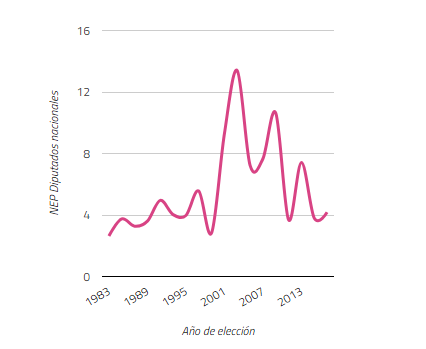
\includegraphics[scale=0.3]{grafico2}
\caption{Indice de independencia judicial}
  \end{figure}
\end{frame}


\begin{frame}\frametitle{Evidencia: Latinoamérica y Argentina (cont.)}
\begin{figure}[htbp]
    \centering
    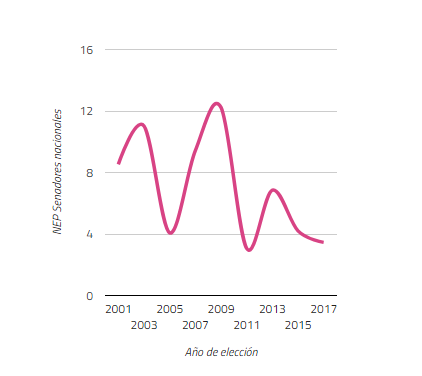
\includegraphics[scale=0.3]{grafico3}
\caption{Independencia judicial y la política económica}
  \end{figure}
\end{frame}


\begin{frame}\frametitle{Evidencia: Latinoamérica y Argentina (cont.)}
Trabajo de Bercoff y Nougués: \medskip 
\begin{itemize}\itemsep 15pt
\item Provincias argentinas para 1991-2001
\item Proceso presupuestario estricto asociado a menor gasto público provincial (per cápita)
\item Provincias con regímenes bicamerales (Corrientes, Entre Ríos, Buenos Aires, Mendoza) tienen menores niveles de gasto per cápita
\item No hay evidencia de correlación significativa entre cláusulas que limitan la reelección y los niveles de gasto per cápita
\end{itemize}
\end{frame}


\begin{frame}\frametitle{Evidencia: Latinoamérica y Argentina (cont.)}
\begin{figure}[htbp]
    \centering
    \includegraphics[scale=0.3]{tabla2}
  \end{figure}
\end{frame}


\begin{frame}\frametitle{Evidencia: Latinoamérica y Argentina (cont.)}
\begin{figure}[htbp]
    \centering
    \includegraphics[scale=0.3]{tabla3}
  \end{figure}
\end{frame}




\end{document}





\begin{frame}\frametitle{Un cuento de dos ciudades}
  \begin{itemize}\itemsep 10pt
  \item
    \end{itemize}
\end{frame}



\begin{frame}\frametitle{Un cuento de dos ciudades}
  \begin{itemize}\itemsep 10pt
  \item
    \end{itemize}
\end{frame}



  
\end{document}
  